








\begin{figure}[h]
    \centering
    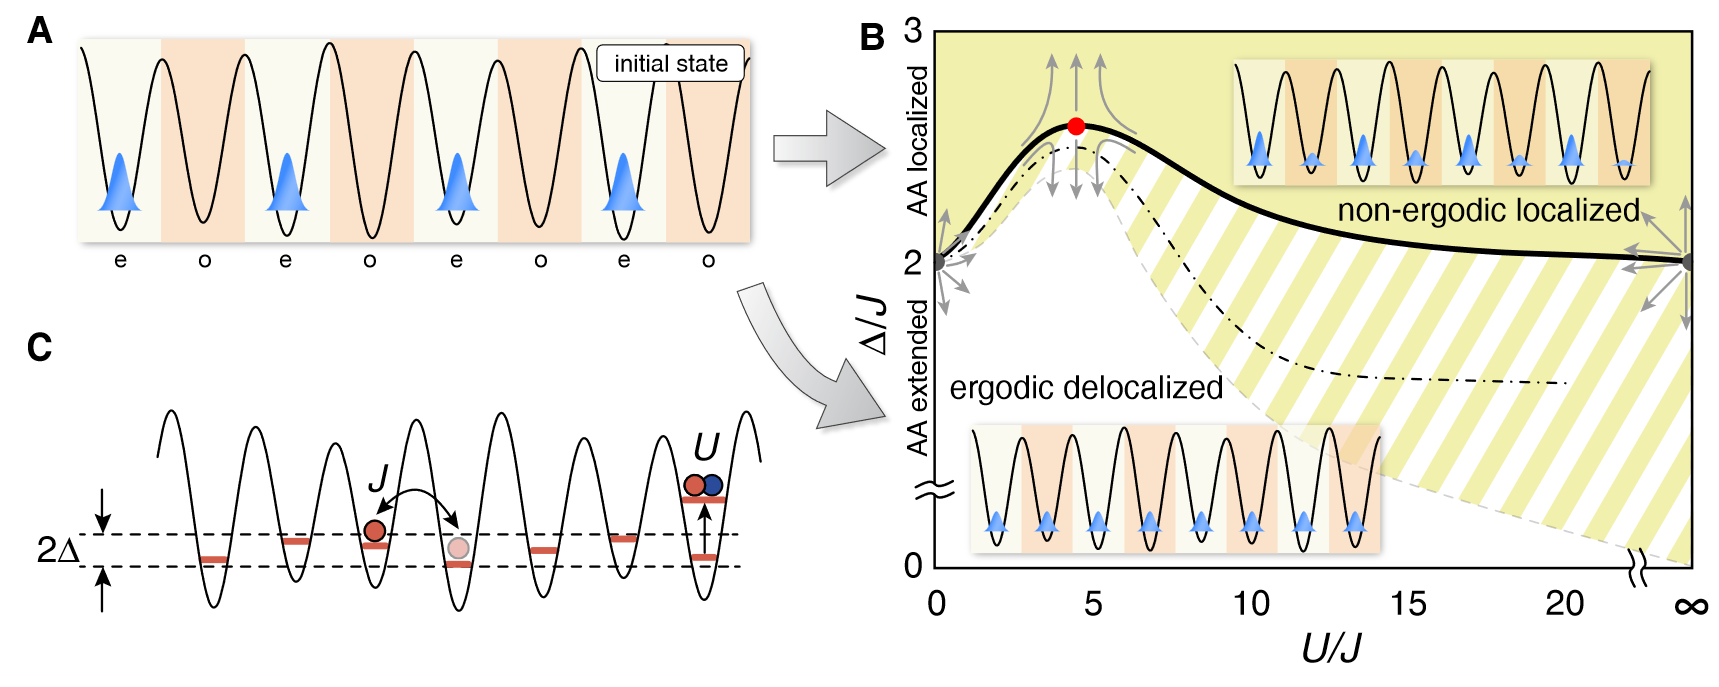
\includegraphics[width=0.7\textwidth]{imgs/1d_phases.png}
    \caption{\cite{schreiber_observation_2015} 1D system \eqref{9:model}. a) Initial state of the system consisting of a charge density wave, where all atoms occupy even sites only. For an interacting many-body system, the evolution of this state over time depends on whether the system is ergodic or not. b) Schematic phase diagram for the system: in the ergodic, delocalized phase (white) the initial state quickly decays, while it persists for long times in the non-ergodic, localized phase (yellow). c) Schematic showing a visual representation of the three terms in the Hamiltonian \eqref{9:model}. }
    \label{fig:1Dmain}
\end{figure}






\begin{figure}[h]
    \centering
    \addletter{75}{a} 
    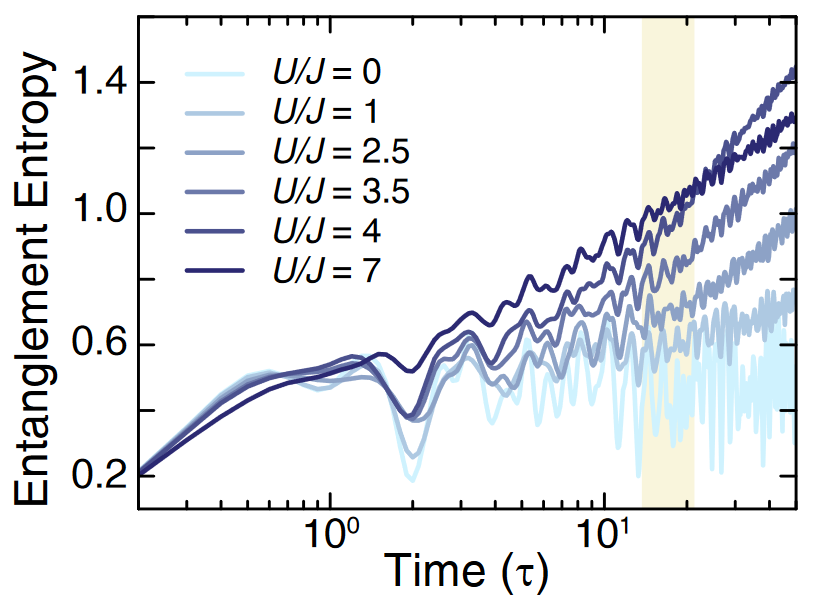
\includegraphics[align=c, width=0.35\textwidth]{imgs/1d_add1.png}
    \hspace{10 mm} 
    \addletter{75}{b} 
    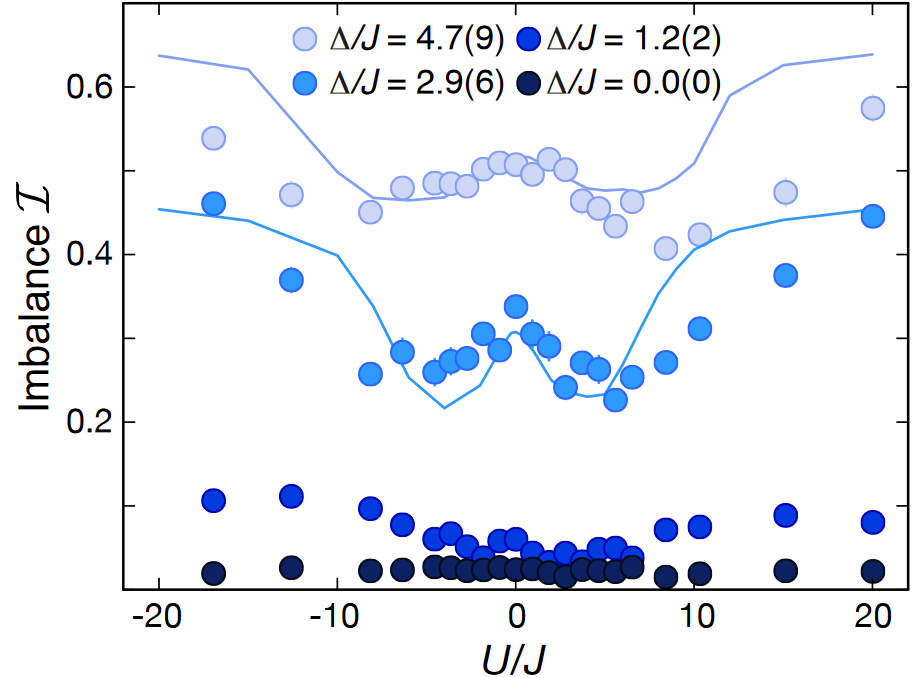
\includegraphics[align=c, width=0.4\textwidth]{imgs/1d_add2.png}
    \caption{
    \cite{schreiber_observation_2015}
        a) DMRG results of the entanglement entropy growth for various interaction strengths and $\Delta = 5 J$. For long times, logarithmic growth characteristic of interacting MBL states is visible.
        b) Cuts along four different disorder strengths. The effect of interactions on the localization gives rise to a characteristic W-shape. Solid lines are the results of DMRG simulations for a single homogeneous tube. 
    }
    \label{fig:1daddb}
\end{figure}

